\documentclass[a4paper, 12pt]{article}
\usepackage[left=2cm,right=2cm,top=2cm,bottom=2cm]{geometry}
\setlength{\parindent}{1cm}
\usepackage{graphicx}
\usepackage{kvsetkeys}
\begin{document}

\title{MM2090 Assignment 4}
\author{Albin George MM20B005}
\date{June 2021}
\maketitle

\section{The Equation}

The Coulombs Law  :  

\begin{equation}
 {\LARGE{\textbf{$F =\frac{Kq1q2}{{r^2}}$}}}
 \label{eqn:equation}
\end{equation}


\subsection{Analysis}
Following contains a brief explanation of the variables and the importance of the equation :
\begin{itemize}

    {\normalsize {The above given equation \ref{eq:1}  has terms \textbf{F} ,\textbf{K} , \textbf{q1},\textbf{q2} and \textbf{r}.}}

{\normalsize { Here,}}\\
{\normalsize {\textbf{F} represents the force exerted by m1 on m2 or vice versa }}\\
{\normalsize {\textbf{K} \  represents the Coulombs Constant}}\\
{\normalsize {\textbf{q1} \  represents the Charge of entity 1}}\\
{\normalsize {\textbf{q2} \  represents the Charge of entity 2}}\\
{\normalsize{\textbf{r} \ represents the distance between entity 1 and entity 2}}
\end{itemize}


Coulomb's law, or Coulomb's inverse-square law, is an experimental law[1] of physics that quantifies the amount of force between two stationary, electrically charged particles. The electric force between charged bodies at rest is conventionally called electrostatic force or Coulomb force.The law was first discovered in 1785 by French physicist Charles-Augustin de Coulomb, hence the name. Coulomb's law was essential to the development of the theory of electromagnetism, maybe even its starting point, as it made it possible to discuss the quantity of electric charge in a meaningful way.

\begin{figure}[h]
	{\begin{center}
		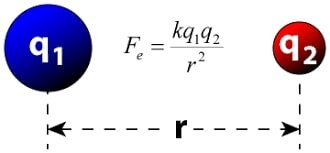
\includegraphics[scale=0.3]{MM20B005.jpg}
	\end{center}}
	\caption{The Coulombs Law\cite{picture}}
	\label{f1:image}
\end{figure}

Webpage Links \cite{website}



%\bibliography{bibliography.bib}
%\bibliographystyle{plain}

\end{document}
